\subsection{Constraints on the dark energy}
Luminosity distance can be written as
\begin{equation}
    d_L = c(1+z)  \int_{0}^{z} \frac{1}{H(z)} dz
\end{equation}
For flat $\Lambda$CDM, $H(z)$ can be written as
\begin{align}
    \label{eq4} H(z) &= H_0 \sqrt{\Omega_M (1+z)^2 + 1 - \Omega_M}
\end{align}
We use emcee\cite{emcee} to fit the dark energy equation. With the Pantheon dataset, the matter density of the flat $\Lambda$CDM model is constrained to be $\Omega_M=0.278 \pm 0.007$. With 24 long GRBs alone, the matter density is constrained to be $\Omega_M=0.307 \pm 0.065$. It indicates that the Hubble diagram in high redshift is consistent with the $\Lambda$CDM model
\begin{figure}[H]
	\centering
	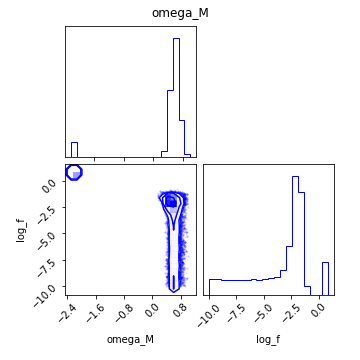
\includegraphics[width=0.5\textwidth]{pantheon/gp/18_omega_M_corner_plot.png}
	\caption{GRB Hubble Diagram}
	\label{fig:OmegaM_GP}
\end{figure}

